\documentclass[12pt,a4paper]{article}

\usepackage{iftex}
\ifPDFTeX
  \usepackage[utf8]{inputenc}
  \usepackage[T2A]{fontenc}
\else
  \usepackage{fontspec}
  \setmainfont{cmunrm.otf}[Path=fonts/,BoldFont=cmunbx.otf,ItalicFont=cmunti.otf,BoldItalicFont=cmunbi.otf]
  \setmonofont{cmuntt.otf}[Path=fonts/,BoldFont=cmuntb.otf,ItalicFont=cmunit.otf,BoldItalicFont=cmuntx.otf]
\fi
\usepackage[russian]{babel}
\usepackage{amsmath}
\usepackage{amssymb}
\usepackage{array}
\usepackage{booktabs}
\usepackage{caption}
\usepackage{enumitem}
\usepackage{fancyhdr}
\usepackage{float}
\usepackage{geometry}
\usepackage{graphicx}
\usepackage{xurl}
\usepackage{hyperref}
\usepackage{indentfirst}
\usepackage{listings}
\usepackage{longtable}
\usepackage{microtype}
\setlength{\emergencystretch}{2em}
\usepackage{xcolor}

\geometry{left=30mm,right=15mm,top=20mm,bottom=20mm}
\setlength{\parindent}{1.25cm}
\linespread{1.2}
\pagestyle{fancy}
\fancyhf{}
\fancyfoot[C]{\thepage}
\renewcommand{\headrulewidth}{0pt}
\hypersetup{hidelinks}

\captionsetup{justification=centering}
\setcounter{tocdepth}{2}

\definecolor{codebg}{RGB}{248,248,248}
\definecolor{codeframe}{RGB}{215,215,215}
\definecolor{codekw}{RGB}{0,76,153}
\definecolor{codestr}{RGB}{163,21,21}
\definecolor{codecomment}{RGB}{0,128,0}
\lstset{
  language=Java,
  basicstyle=\ttfamily\small,
  keywordstyle=\color{codekw}\bfseries,
  stringstyle=\color{codestr},
  commentstyle=\color{codecomment},
  backgroundcolor=\color{codebg},
  frame=single,
  rulecolor=\color{codeframe},
  numbers=left,
  numberstyle=\tiny,
  stepnumber=1,
  breaklines=true,
  showstringspaces=false,
  tabsize=2,
  columns=fullflexible,
  keepspaces=true,
  extendedchars=true,
  inputencoding=utf8,
  upquote=true
}

\newcolumntype{C}[1]{>{\centering\arraybackslash}p{#1}}


% Данные титульного листа. Номер работы не задан: при необходимости добавьте его.
\newcommand{\LabTitle}{Лабораторная работа}
\newcommand{\StudentName}{Якименко Владислав Игоревич}
\newcommand{\StudentGroup}{P3313}
\newcommand{\TeacherName}{Кобик Никита Алексеевич}

\begin{document}
\pagenumbering{gobble}
\hypersetup{pageanchor=false}
\begin{titlepage}
  \thispagestyle{empty}
  \begin{center}
    {\small Федеральное государственное автономное образовательное учреждение высшего образования\\
    «Национальный исследовательский университет ИТМО»}\\[0.8em]
    {\small Факультет программной инженерии и компьютерной техники}

    \vfill

    {\Large\textbf{\LabTitle}}\\[0.6em]
    {\large «Информационная система\\управления фильмами»}\\[0.6em]
    {\large по курсу «Информационные системы»}\\[0.6em]
    {\large Вариант 53434963}

    \vfill

    \begin{flushright}
      \begin{tabular}{l}
        Выполнил:\\
        \StudentName, \StudentGroup\\[0.8em]
        Проверил:\\
        \TeacherName
      \end{tabular}
    \end{flushright}

    \vfill

    Санкт-Петербург --- 2026
  \end{center}
\end{titlepage}
\clearpage
\hypersetup{pageanchor=true}
\tableofcontents
\thispagestyle{empty}
\clearpage
\pagenumbering{arabic}
\section{Цель работы и текст задания}


Цель работы — разработать многопользовательскую информационную систему для управления фильмами и связанными объектами с использованием Jakarta EE, CDI, \path{JPA/Hibernate} и PostgreSQL. Ниже приведён текст индивидуального задания для варианта 53434963.


Реализовать информационную систему, которая позволяет взаимодействовать с объектами класса Movie, описание которого приведено ниже:


\lstinputlisting[language=Java,basicstyle=\ttfamily\footnotesize,numbers=none]{model-spec.java}


Разработанная система должна удовлетворять следующим требованиям:


\begin{itemize}[leftmargin=*]

\item Основное назначение информационной системы - управление объектами, созданными на основе заданного в варианте класса.

\item Необходимо, чтобы с помощью системы можно было выполнить следующие операции с объектами: создание нового объекта, получение информации об объекте по ИД, обновление объекта (модификация его атрибутов), удаление объекта. Операции должны осуществляться в отдельных окнах (интерфейсах) приложения. При получении информации об объекте класса должна также выводиться информация о связанных с ним объектах.

\item При создании объекта класса необходимо дать пользователю возможность связать новый объект с объектами вспомогательных классов, которые могут быть связаны с созданным объектом и уже есть в системе.

\item Выполнение операций по управлению объектами должно осуществляться на серверной части (не на клиенте), изменения должны синхронизироваться с базой данных.

\item На главном экране системы должен выводиться список текущих объетов в виде таблицы (каждый атрибут объекта - отдельная колонка в таблице). При отображении таблицы должна использоваться пагинация (если все объекты не помещаются на одном экране).

\item Нужно обеспечить возможность фильтровать/сортировать строки таблицы, которые показывают объекты (по значениям любой из строковых колонок). Фильтрация элементов должна производиться по неполному совпадению.

\item Переход к обновлению (модификации) объекта должен быть возможен из таблицы с общим списком объектов и из области с визуализацией объекта (при ее реализации).

\item При добавлении/удалении/изменении объекта, он должен автоматически появиться/исчезнуть/измениться в интерфейсах у других пользователей, авторизованных в системе.

\item Если при удалении объекта с ним связан другой объект, связанные объекты должны удаляться.

\item Пользователи должны иметь возможность просмотра всех объектов. Для модификации объекта должно открываться отдельное диалоговое окно. При вводе некорректных значений в поля объекта должны появляться информативные сообщения о соответствующих ошибках.

\end{itemize}

В системе должен быть реализован отдельный пользовательский интерфейс для выполнения специальных операций над объектами:


\begin{itemize}[leftmargin=*]

\item Удалить один (любой) объект, значение поля tagline которого эквивалентно заданному.

\item Вернуть массив объектов, значение поля tagline которых содержит заданную подстроку.

\item Вернуть массив объектов, значение поля genre которых меньше заданного.

\item Получить список сценаристов, ни один фильм которых не получил ни одного "Оскара".

\item Равномерно перераспределить все "Оскары", полученные фильмами одного жанра, между фильмами другого жанра.

\item Представленные операции должны быть реализованы в качестве функций БД, которые необходимо вызывать из уровня бизнес-логики приложения.

\end{itemize}

Особенности хранения объектов, которые должны быть реализованы в системе:


\begin{itemize}[leftmargin=*]

\item Организовать хранение данных об объектах в реляционной СУБД (PostgreSQL). Каждый объект, с которым работает ИС, должен быть сохранен в базе данных.

\item Все требования к полям класса (указанные в виде комментариев к описанию классов) должны быть выполнены на уровне ORM и БД.

\item Для генерации поля id использовать средства базы данных.

\item Для подключения к БД на кафедральном сервере использовать хост pg, имя базы данных - studs, имя пользователя/пароль совпадают с таковыми для подключения к серверу.

\end{itemize}

При создании системы нужно учитывать следующие особенности организации взаимодействия с пользователем:


\begin{itemize}[leftmargin=*]

\item Система должна реагировать на некорректный пользовательский ввод, ограничивая ввод недопустимых значений и информируя пользователей о причине ошибки.

\item Переходы между различными логически обособленными частями системы должны осуществляться с помощью меню.

\item При добавлении/удалении/изменении объекта, он должен автоматически появиться/исчезнуть/измениться на области у всех других клиентов.

\end{itemize}

При разработке ИС должны учитываться следующие требования:


\begin{itemize}[leftmargin=*]

\item В качестве основы для реализации ИС необходимо использовать Jakarta EE, CDI beans.

\item Для создания уровня хранения необходимо использовать JPA + Hibernate.

\item Разные уровни приложения должны быть отделены друг от друга, разные логические части ИС должны находиться в отдельных компонентах.

\end{itemize}

\clearpage

\section{UML диаграмма классов}


Показаны предметные сущности, поля и кратности связей. Поля id вспомогательных сущностей и version добавлены для хранения ссылок и контроля конкурирующих изменений. Доступ к приватным полям предоставляется методами, которые для компактности диаграммы не показаны.


\begin{figure}[H]\centering
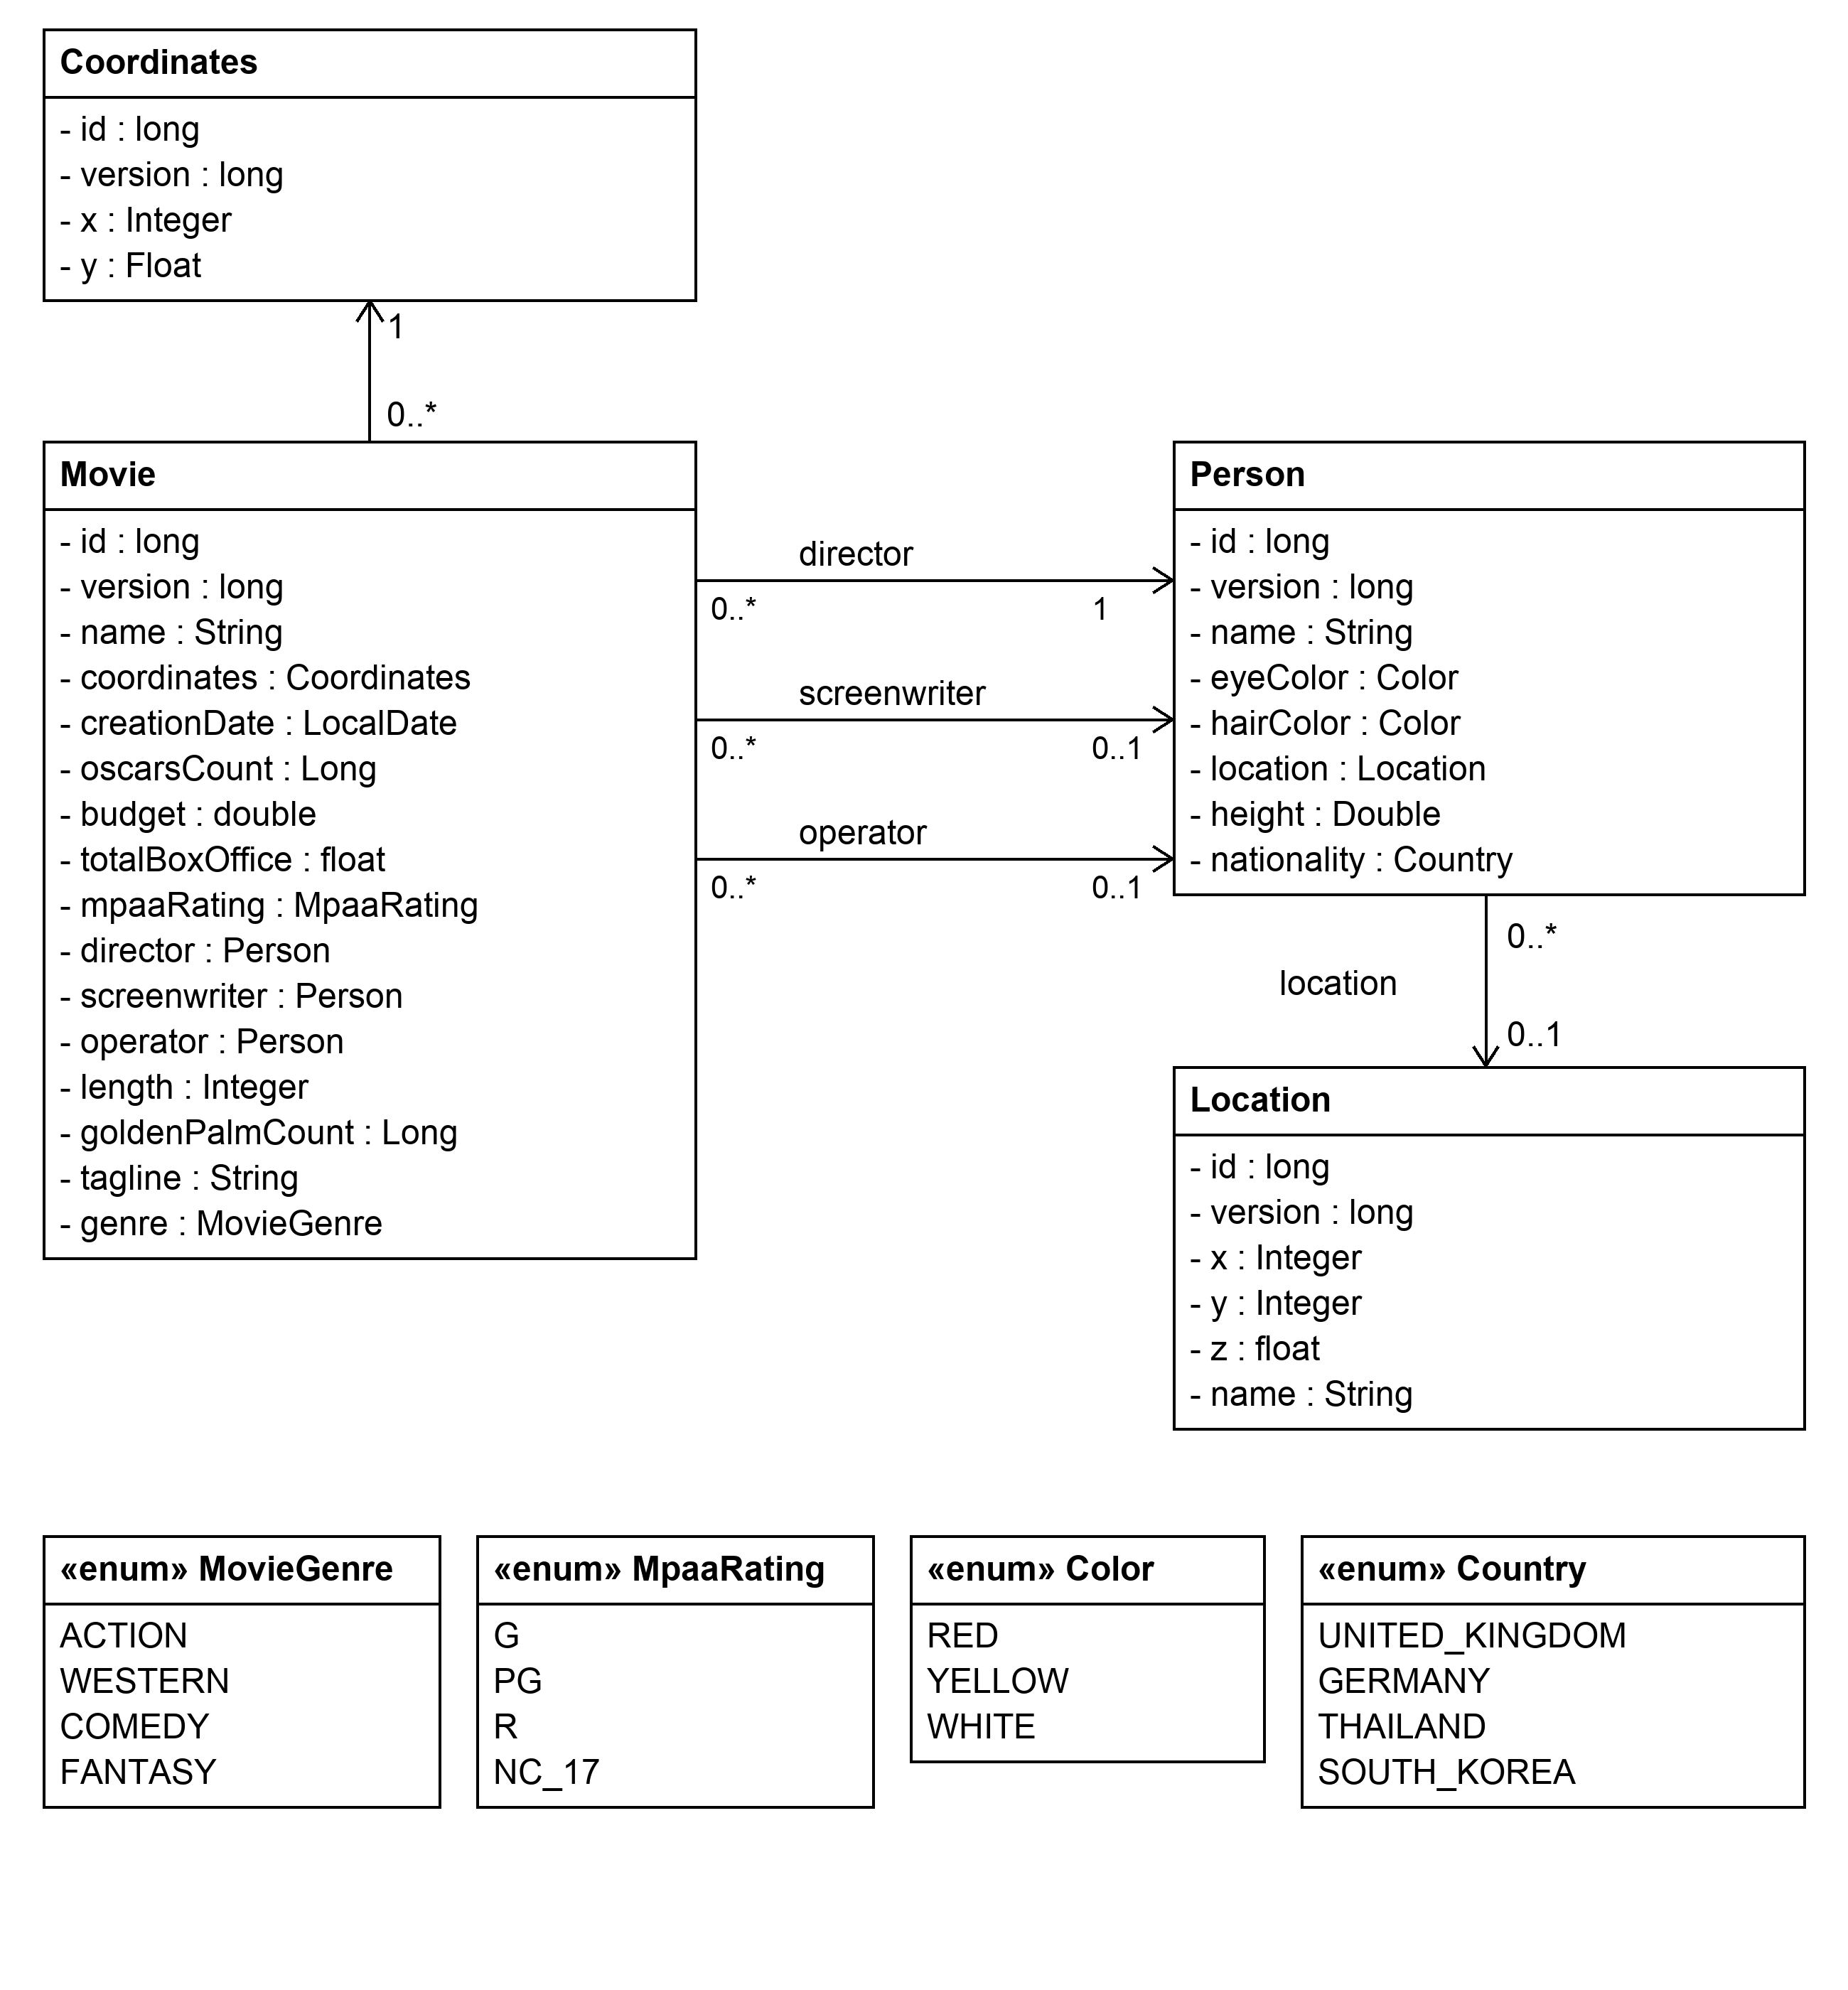
\includegraphics[width=\linewidth,height=0.74\textheight,keepaspectratio]{figures/classes.png}
\caption{Классы предметной области}
\end{figure}

\clearpage

\section{UML диаграмма пакетов}


Диаграмма показывает основные направления вызовов и использования моделей. Вспомогательные зависимости обработки ошибок не показаны. Интерфейс браузера обращается к REST-ресурсам пакета web.


\begin{figure}[H]\centering
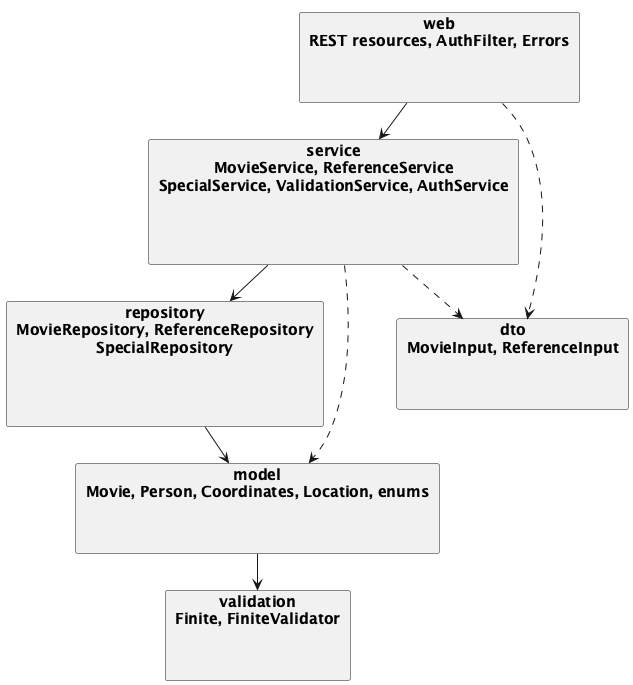
\includegraphics[width=0.78\linewidth,height=0.74\textheight,keepaspectratio]{figures/packages.png}
\caption{Пакеты приложения}
\end{figure}

\clearpage

\section{Исходный код}

Исходный код приложения доступен в публичном репозитории:
\url{https://github.com/delovoyhomie/movie-lab-53434963}.

Серверная часть находится в \path{src/main/java}, интерфейс — в \path{src/main/webapp}, схема базы данных и SQL-функции — в каталоге db.

\section{Выводы}


Реализована информационная система управления фильмами с разделением HTTP-интерфейса, бизнес-логики и доступа к данным. JPA и Hibernate связывают предметные сущности с PostgreSQL, а ограничения Java и базы данных защищают целостность данных независимо от клиентского интерфейса.


Специальные операции выполняются функциями PostgreSQL. Транзакции обеспечивают атомарность перераспределения наград; версии сущностей предотвращают сохранение устаревших форм. Периодический опрос версии модели синхронизирует интерфейсы пользователей. Для небольшого учебного приложения выбраны простая архитектура одного WAR и минимальный интерфейс без дополнительных фреймворков.

\end{document}
